\documentclass[12pt,brazilian,twoside]{abntex2}

\usepackage[utf8]{inputenc} % fonte com acentos
\usepackage{times} % fonte times
\usepackage{indentfirst} % indenta primeiro parágrafo
\usepackage{graphicx} % para utilizar imagens
\usepackage[brazilian,hyperpageref]{backref}     % Paginas com as citações na bibl
\usepackage[alf]{abntex2cite}   % Citações padrão ABNT

\titulo{Meu trabalho de conclusão de curso em LaTeX}
\autor{Diego Cirilo}
\local{Mossoró, RN}
\data{2014}
\orientador{Fulano dos Anzóis}
\coorientador{Sicrano das Iscas}
\instituicao{
Instituto Federal do Rio Grande do Norte - IFRN
\par
Departamento de Danças Folclóricas}
\tipotrabalho{Trabalho de Conclusão de Curso}
\preambulo{Trabalho de Conclusão de Curso apresentado ao Departamento de Danças Folclóricas do IFRN como requisito parcial para obtenção do título de Bacharel em Danças Folclóricas.}

\makeindex % Compila o sumário

\begin{document}
\pretextual

\imprimircapa

\imprimirfolhaderosto

\begin{folhadeaprovacao}
 
  \begin{center}
    {\ABNTEXchapterfont\large\imprimirautor}
 
    \vspace*{\fill}\vspace*{\fill}
    {\ABNTEXchapterfont\bfseries\Large\imprimirtitulo}
    \vspace*{\fill}
   
    \hspace{.45\textwidth}
    \begin{minipage}{.5\textwidth}
        \imprimirpreambulo
    \end{minipage}%
    \vspace*{\fill}
   \end{center}
   
   Trabalho aprovado. \imprimirlocal, 24 de novembro de 2014:
 
   \assinatura{\textbf{\imprimirorientador} \\ Orientador}
   \assinatura{\textbf{Professor Dr. Luiz da Silva} \\ Examinador Interno}
   \assinatura{\textbf{Professor Me. Fernando Salles} \\ Examinador Externo}
   %\assinatura{\textbf{Professor} \\ Convidado 3}
   %\assinatura{\textbf{Professor} \\ Convidado 4}
     
   \begin{center}
    \vspace*{0.5cm}
    {\large\imprimirlocal}
    \par
    {\large\imprimirdata}
    \vspace*{1cm}
  \end{center}
 
\end{folhadeaprovacao}

\begin{dedicatoria}
   \vspace*{\fill}
   \centering
   \noindent
   \textit{ Este trabalho é dedicado às crianças adultas que,\\
   quando pequenas, sonharam em se tornar cientistas.} \vspace*{\fill}
\end{dedicatoria}

\begin{agradecimentos}
Agradeço aos colegas do IFRN que permitiram a execução desse trabalho.
Agradeço também aos colegas do futebol...
\end{agradecimentos}

\begin{epigrafe}
    \vspace*{\fill}
        \begin{flushright}
                \textit{``Não vos amoldeis às estruturas deste mundo, \\
                mas transformai-vos pela renovação da mente, \\
                a fim de distinguir qual é a vontade de Deus: \\
                o que é bom, o que Lhe é agradável, o que é perfeito.\\
                (Bíblia Sagrada, Romanos 12, 2)}
        \end{flushright}
\end{epigrafe}

\begin{resumo}
 Segundo a o resumo deve ressaltar o
 objetivo, o método, os resultados e as conclusões do documento. A ordem e a extensão
 destes itens dependem do tipo de resumo (informativo ou indicativo) e do
 tratamento que cada item recebe no documento original. O resumo deve ser
 precedido da referência do documento, com exceção do resumo inserido no
 próprio documento. (\ldots) As palavras-chave devem figurar logo abaixo do
 resumo, antecedidas da expressão Palavras-chave:, separadas entre si por
 ponto e finalizadas também por ponto.
 
 \vspace{\onelineskip}
   
 \noindent
 \textbf{Palavras-chaves}: latex. abntex. editoração de texto.
\end{resumo}
 
% resumo em inglês
\begin{resumo}[Abstract]
 \begin{otherlanguage*}{english}
   This is the english abstract.
 
   \vspace{\onelineskip}
 
   \noindent
   \textbf{Key-words}: latex. abntex. text editoration.
 \end{otherlanguage*}
\end{resumo}

% ---
% inserir lista de ilustrações
% ---
\pdfbookmark[0]{\listfigurename}{lof}
\listoffigures*
\cleardoublepage
% ---
 
% ---
% inserir lista de tabelas
% ---
\pdfbookmark[0]{\listtablename}{lot}
\listoftables*
\cleardoublepage
% ---
 
% ---
% inserir lista de abreviaturas e siglas
% ---
\begin{siglas}
  \item[Fig.] Area of the $i^{th}$ component
  \item[456] Isto é um número
  \item[123] Isto é outro número
  \item[lauro cesar] este é o meu nome
\end{siglas}
% ---
 
% ---
% inserir lista de símbolos
% ---
\begin{simbolos}
  \item[$ \Gamma $] Letra grega Gama
  \item[$ \Lambda $] Lambda
  \item[$ \zeta $] Letra grega minúscula zeta
  \item[$ \in $] Pertence
\end{simbolos}
% ---
 
% ---
% inserir o sumario
% ---
\pdfbookmark[0]{\contentsname}{toc}
\tableofcontents*
\cleardoublepage
% ---

\textual
\chapter{Introdução}
É com muita alegria que inicio este trabalho \cite{ortega2010ritalina}. 

Segundo \citeonline{ortega2010ritalina} podemos analisar os dados..
\section{Metodologia}
Os métodos do pato da Figura \ref{pato}
\begin{figure}[h]
\center
\caption{O pato interessante.}
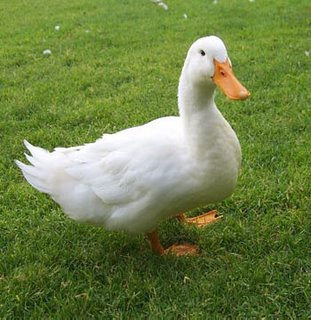
\includegraphics[width=6cm]{pato}
\legend{Fonte: FERNANDES,2014}
\label{pato}
\end{figure}

\chapter{Referencial Teórico}
 
 Bla bla bla, como é possível observar na Tabela \ref{usuarios}...
\begin{table}[h]
\center
\caption{Tabela dos Usuários}
\begin{tabular}{|l|l|l|l|}
\hline
Idade & A1    & A2   & A3   \\ \hline
Nome  & Diego & João & Luiz \\ \hline
\end{tabular}
\label{usuarios}
\legend{Fonte: \cite{ortega2010ritalina}}
\end{table}

\chapter{Procedimentos}

\chapter{Resultados}

\chapter{Conclusão}

\postextual

\bibliography{bibliografia}

\anexos
\chapter{Exemplo de anexo}

\end{document}